\documentclass{article}

\usepackage{multicol}
\usepackage{amsmath}
\usepackage{tikz}
\usetikzlibrary{bayesnet}

\begin{document}

\begin{multicols}{2}
  \begin{align*}
    y_i &\sim Poisson(\lambda_i)\\
    ln(\lambda_i) &= a_{p[i]} + \tilde{f}_{g[i],p[i]} + f_{g[i]}\\
    \\
    a_{p[i]} &= \mu + \sigma * z_{p[i]} \\
    \mu &\sim Unif(-\infty, \infty) \\
    \sigma &\sim \mathcal{N}(0, 1) \\
    z_{p[i]} &\sim \mathcal{N}(0, 1) \\
    \\
    \boldsymbol{f} &\sim GP(0, K_{\rho, \alpha}) \\
    \rho &\sim InvGamma(10, 500) \\
    \alpha &\sim \mathcal{N}(0, 1) \\
    \\
    \boldsymbol{\tilde{f}_{p[i]}} &\sim GP(0, K_{\tilde{\rho}, \tilde{\alpha}}) \\
    \tilde{\rho} &\sim InvGamma(20, 600) \\
    \tilde{\alpha} &\sim \mathcal{N}(0, 1) \\
  \end{align*}
  
  \columnbreak
  
  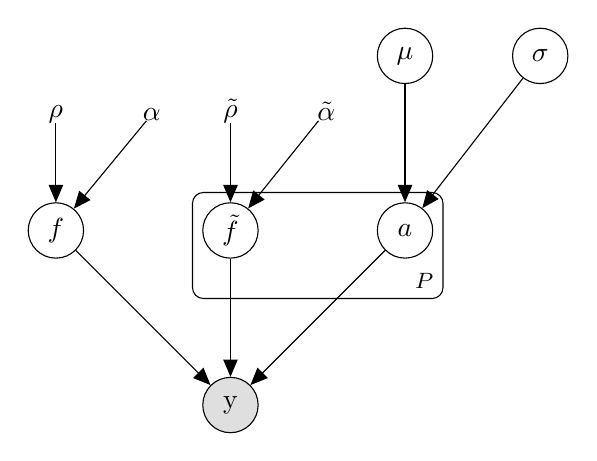
\begin{tikzpicture}
    \node[obs, yshift=1cm] (y) {y};
    \node[latent, above=of y, yshift=0.5cm] (ft) {$\tilde{f}$};
    \node[latent, left=of ft, xshift=-.5cm] (f) {$f$};
    \node[latent, right=of ft, xshift=.5cm] (a) {$a$};
    
    \node[latent, above=of a, yshift=0.5cm] (mu) {$\mu$};
    \node[latent, right=of mu] (sd) {$\sigma$};
    
    \node[const, above=of ft] (rhot) {$\tilde{\rho}$};
    \node[const, right=of rhot] (alphat) {$\tilde{\alpha}$};
    \node[const, above=of f] (rho) {$\rho$};
    \node[const, right=of rho] (alpha) {$\alpha$};
    
    
    \edge {rho, alpha} {f}
    \edge {rhot, alphat} {ft}
    \edge {mu, sd} {a}
    \edge {a, ft, f} {y}
    
    \plate {p} {(ft)(a)} {$P$}
  \end{tikzpicture}
  
\end{multicols}
\end{document}
